\begin{figure}[H]
  \centering
  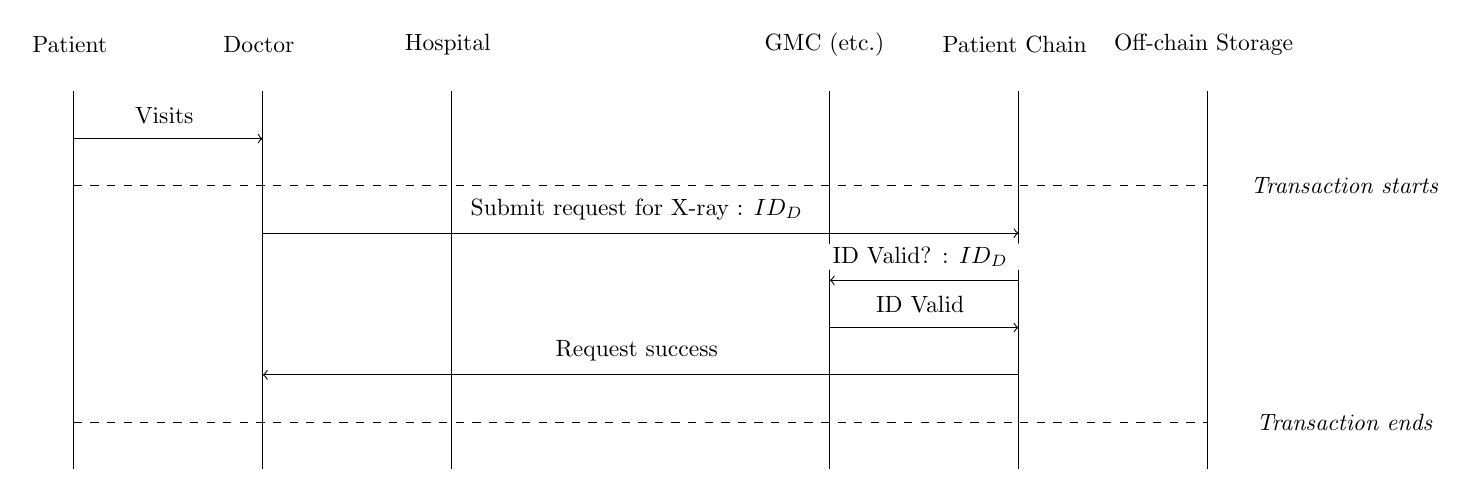
\begin{tikzpicture}[scale = 0.6, every node/.style={scale = 0.85}, every node/.append style={fill = white, rounded corners = 2pt, inner sep = 2pt, align = center}]

  % Lines
  \draw (4, 12) -- (4, 20);
  \draw (8, 12) -- (8, 20);
  \draw (12, 12) -- (12, 20);
  \draw (20, 12) -- (20, 20);
  \draw (24, 12) -- (24, 20);
  \draw (28, 12) -- (28, 20);

  % Headings
  \node at (4, 21) { Patient };
  \node at (8, 21) { Doctor };
  \node at (12, 21) { Hospital };
  \node at (20, 21) { GMC (etc.) };
  \node at (24, 21) { Patient Chain };
  \node at (28, 21) { Off-chain Storage };

  % Arrows
  \node at (6, 19.5) { Visits };
  \draw [ -> ] (4, 19) -- (8, 19);

  \node at (31, 18) { \textit{Transaction starts} };
  \draw [ dashed ] (4, 18) -- (28, 18);

  \node at (16, 17.5) { Submit request for X-ray : $ID_{D}$ };
  \draw [ -> ] (8, 17) -- (24, 17);

  \node at (22, 16.5) { ID Valid? : $ID_{D}$ };
  \draw [ -> ] (24, 16) -- (20, 16);

  \node at (22, 15.5) { ID Valid \checkmark };
  \draw [ -> ] (20, 15) -- (24, 15);

  \node at (16, 14.5) { Request success };
  \draw [ -> ] (24, 14) -- (8, 14);

  \node at (31, 13) { \textit{Transaction ends} };
  \draw [ dashed ] (4, 13) -- (28, 13);

  \end{tikzpicture}
  \caption{
    Doctor requests patient X-ray
  }{
    The doctor sends a transaction to the patient's record which creates a request file with the details of what needs to be done and the doctors notes. This will need to be accepted by the hospital.
  }
  \label{fig:user_story_01a}
\end{figure}
